\documentclass[a4paper]{article}

\usepackage[T3]{fontenc}
\usepackage[utf8]{inputenc}
\usepackage[russian]{babel}

\usepackage{fullpage} % Package to use full page
\usepackage{parskip} % Package to tweak paragraph skipping

\usepackage{amsmath, amssymb}
\usepackage{graphicx}
\usepackage[colorinlistoftodos]{todonotes}

\usepackage{gensymb} % для значка градуса

\usepackage[nottoc]{tocbibind}

\usepackage{mhchem}

\begin{document}

\begin{titlepage}
\centering
\textbf{\large Московский государственный университет имени М.В.\,Ломоносова\\
\vspace*{0.1cm} Химический факультет\\
\vspace*{0.1cm}
\noindent\makebox[\linewidth]{\rule{\paperwidth}{0.4pt}}
\vspace*{0.1cm}
 Кафедра органической химии\\
\vspace*{0.1cm} Лаборатория супрамолекулярной химии и нанотехнологии органических материалов \\}
\vspace*{2cm}

\begin{center}

\includegraphics[width=0.3\textwidth]{pictures/logo.jpg}
\end{center}

\vspace*{2cm}
\Large \textbf{Отчет.}
\vspace*{2cm}

\begin{flushright}
Научный руководитель:\\
к.х.н., доц. Нуриев В.Н.
\end{flushright}
\vfill
\large\textbf{Москва\\ 2016}
\end{titlepage}

\tableofcontents

\section{Синтез 2-бензилиденциклопентанона.}
\begin{center}
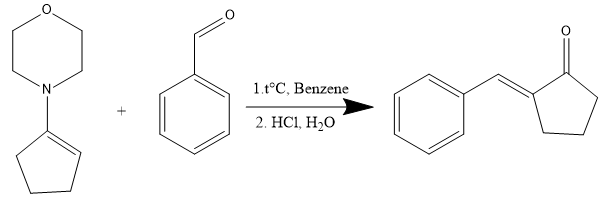
\includegraphics[scale=0.5]{pictures/1.png}
\end{center}
11.45г (74.84 ммоль) N-циклопентенилморфолина, 6.61г (62.36 ммоль) свежеперегнанного бензальдегида и 60 мл бензола помещают в круглодонную колбу и нагревают с насадкой Дина-Старка в течение 20 часов. За ходом реакции следят при помощи ТСХ (элюент -- петролейный эфир : этилацетат, 4 : 1).
Затем раствор охлаждают до комнатной температуры и при перемешивании добавляют 43.5 мл 6М $\ce{HCl}$. После перемешивания в течение 2 часов органический слой отделяют и промывают водой до нейтрального pH, оставляют сушиться над $\ce{Na2SO4}$ на ночь. Затем смесь фильтруют и отгоняют бензол на роторном растворителе. Остаток представляет собой темное масло, которое кристаллизуется при затирании палочкой. Очистку производят перекристаллизацией из циклогексана. Выход: 4.8г (44.75\%).\\
Температура плавления очищенного вещества: $T_{melt.} = 62 - 63^{\circ}$С. $T_{melt.}^{lit.} = 60 - 62^{\circ}$C \cite{takeishi2004} \\
Спектр ЯМР $^{1}$H ($\ce{CDCl3}$, 400 МГц, $\delta$ м.д., \textit{J} Гц):   2.02 (2H, квинт., \textit{J} = 7.8 Гц, H(1)), 2.40 (2H, т, \textit{J} = 7.8 Гц, H(2)), 2.97 (2H, дт, \textit{J} = 2.5 Гц, H(5)), 7.40 (4H, м, H(10),H(11),H(12),H(7)), 7.52 (2H, д, \textit{J} = 7.3 Гц, H(9), H(13)). 

\section{Синтез 2-бензилиден-5-(4-метоксибензилиден)циклопентанона.}
\begin{center}
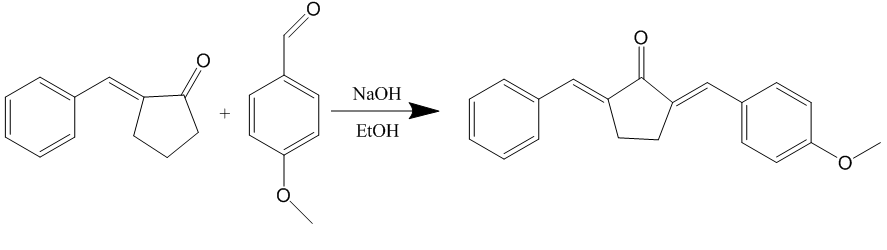
\includegraphics[scale=0.35]{pictures/2.png}
\end{center}
172 мг  моноенона, 136 мг анисового альдегида, 230 мкл 2N $\ce{NaOH}$ и 1.5мл $\ce{EtOH}$ помещают в круглодонную колбу и перемешивают в течение часа. Реакция протекает при комнатной температуре, за ходом реакции следят при помощи ТСХ. Реакция сопровождается выпадением грязно-желтого осадка диенона. После окончания реакции реакционную смесь переносят на фильтр со стеклянным фильтрующим дном, осадок промывают небольшими количествами воды, сушат в пистолете Фишера. Выход: 118 мг (40.69$\%$). \\
$T_{melt.} = 169-170^{\circ}$С. $T_{melt.}^{lit.} = 170-171^{\circ}$C. \cite{rosamilia2006} \\
Спектр ЯМР$^{1}$Н ($\ce{CDCl3}$, 400 МГц, $\delta$ м.д., \textit{J} Гц): 3.12 (4H, ушир. с, H(3), H(4)), 3.87 (3H, с, H(22)), 6.99 (2H, д, \textit{J} = 8.69 Гц, H(10), H(12)), 7.37 (1H, м, H(18), 7.45 (2H, м, H(17), H(19)), 7.60 (6H, м, H(16),H(20),H(9),H(13),H(7),H(14)).

\section{Синтез 2-бензилиден-5-(пиридин-3-илметилен)циклопентанона.}
\begin{center}
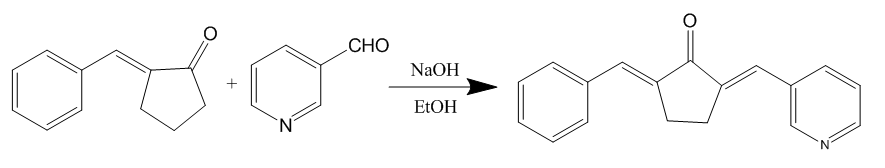
\includegraphics[scale=0.35]{pictures/3.png}
\end{center}
172 мг моноенона, 107 мг 3-пиридинкарбальдегида, 330 мкл 2N $\ce{NaOH}$ и 1.5 мл $\ce{EtOH}$ помещают в круглодонную колбу и перемешивают в течение часа. Реакция протекает при комнатной температуре, за ходом реакции следят при помощи ТСХ. Реакция сопровождается выпадением оранжево-желтого осадка диенона. После окончания реакции реакционную смесь переносят на фильтр со стеклянным фильтрующим дном, осадок промывают небольшими количествами воды, сушат в пистолете Фишера. Выход: 117 мг (44.83$\%$). \\
$T_{melt.} = 187-188^{\circ}$С. $T_{melt.}^{lit.} = 198^{\circ}$C. \cite{vatsadze2005} \\
Спектр ЯМР$^{1}$H ($\ce{CDCl3}$, 400 МГц, $\delta$ м.д., \textit{J} Гц): 3.15 (4H, ушир. с, H(11), H(12)), 7.42 (4H, м, H(17), H(18), H(19), H(3)), 7.56 (1H, с, H(14)), 7.65 (3H, м, H(16), H(20), H(7)), 7.91 (1H, д, \textit{J} = 8.1 Гц, H(4)), 8.61 (1H, д, \textit{J} = 4.5 Гц, H(6)), 8.86 (1H, с, H(2))

\section{Синтез бензил-1,4-диил-диметилидендициклопентанона.}
\begin{center}
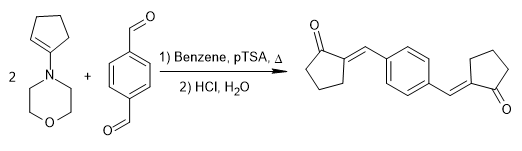
\includegraphics[scale=0.45]{pictures/4.png}
\end{center}
К раствору 50 ммоль N-циклопентенморфолина в 50 мл бензола добавляют 2-3 капли морфолина и 50 мг п-толуолсульфокислоты. Смесь кипятят с насадкой Дина-Старка до прекращения выделения воды (30-60 минут). Затем к смеси добавляют 25 ммоль терефталевого альдегида, интенсивно перемешивают и кипятят с азеотропной отгонкой воды 12-14 часов, в результате чего получается черная смолообразная смесь. После охлаждения к смеси прибавляют 20 мл конц. $\ce{HCl}$ и перемешивают при 20$^{\circ}$ в течение 3 часов. Продукт экстрагируют $\ce{CH2Cl2}$, объединенные вытяжки сушат над $\ce{Na2SO4}$ и упаривают в роторном испарителе. Затем готовят смесь остатка с минимальным количеством силикагеля (до получения пересыпчатого порошка) и проводят флэш-хроматографию с элюентом $\ce{EtOAC}$ - $\ce{C6H14}$ (с плавным возрастанием полярности от 1:5 до 3:1). Получают 34.89$\%$ целевого диенона. Выход: 2.32 г (34.89 $\%$).
$T_{melt.} = 181-184^{\circ}$С. $T_{melt.}^{lit.} = 185^{\circ}$C \cite{dimmock2002} \\
Спектр ЯМР$^{1}$H ($\ce{CDCl3}$, 400 МГц, $\delta$ м.д., \textit{J} Гц): 2.04 (4H, квинт. H(18), H(1)), 2.40 (4H, т, \textit{J} = 7.9 Гц, H(17), H(2)), 2.98 (4H, тд, \textit{J} = 7.14, 2.15 Hz, H(19), H(5)), 7.35 (2H, т, \textit{J} = 2.57 Гц, H(7), H(14)), 7.56 (4H, с, H(9), H(10), H(12), H(13)).

\bibliographystyle{unsrt}
\bibliography{sample}

\end{document}